%!TEX root = iclr2026_conference.tex
% Appendix A (sec:app:notation): description-level example (fig:levels), notation, glossary, time base, arm key.
% Content plan and owner unit: manuscript/paper-contract.md §8.
\section{\texorpdfstring{\rev{Notation, Glossary and Arm Key}}{Notation, Glossary and Arm Key}}
\label{sec:app:notation}

\begin{revblock}\nopagebreak
This appendix collects a real-frame example of the description levels, the symbols, terms and time units, and the arm names used throughout the paper. Record names and ticket numbers (\#NNN) identify the experiment records listed in Appendix~\ref{sec:app:repro}.

\subsection{Description levels on a real frame}

Figure~\ref{fig:levels} shows the three description levels of Section~\ref{sec:mth:setting} on one recorded NovPhy frame.
\end{revblock}

\begin{figure}[H]
\centering
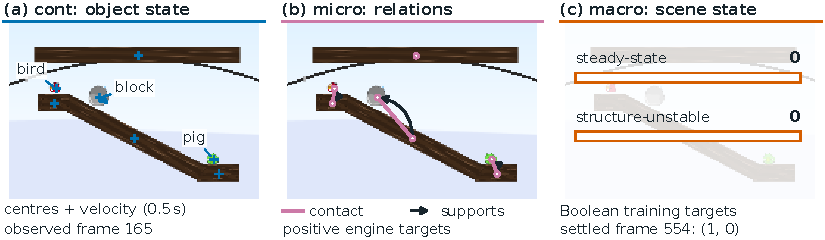
\includegraphics[width=\linewidth]{figures/fig_description_levels.pdf}
\caption[Three description levels on one real frame]{\textbf{Three description levels on one real frame.} A NovPhy frame during the cascade, described at each level $\alpha$. (a) $\textsf{cont}$: each object's centre and velocity. (b) $\textsf{micro}$: objects in contact (lines) and support relations (arrows, from supporter to supported). (c) $\textsf{macro}$: two scene predicates, both false here; once the scene settles (frame 554), steady-state becomes true. All panels show engine states and the engine labels used as training targets, not model outputs. \rev{The figure illustrates training targets. It is not evidence that the model's predicted $\textsf{micro}$ or $\textsf{macro}$ predicates stay accurate during a rollout (Section~\ref{sec:disc}).}}
\label{fig:levels}
\end{figure}

\begin{revblock}
\subsection{Notation}

Table~\ref{tab:app:notation} lists the symbols. In Sections~\ref{sec:mth:setting}--\ref{sec:mth:model}, $t$ indexes engine steps and $k$ carrier frames. From Section~\ref{sec:mth:protocol} on, $t$ also counts carrier frames from the decision frame, so $t=225$ is the NovPhy rollout endpoint $K$.
\end{revblock}

\begin{table}[H]
\ifshowrevisions\color{blue}\fi
\centering
\footnotesize
\caption{Notation.}
\label{tab:app:notation}
\begin{tabular}{@{}>{\raggedright\arraybackslash}p{0.24\linewidth}>{\raggedright\arraybackslash}p{0.7\linewidth}@{}}
\toprule
Symbol & Meaning \\
\midrule
$s$, $a$, $o_t$ & Decision state (a NovPhy level at its decision frame), launch, RGB observation \\
$\mathcal{C}(s)$ & Inventory: the candidate launches of a level \\
$y(s,a)\in\{0,1\}$ & Engine outcome: 1 when the engine removes the pig at the first shot \\
$E$ & Frozen object-slot encoder \\
$z_k$, $\hat z_k$, $\tilde z_k$ & Observed carrier, predicted carrier, and fixed DP context carrier at carrier frame $k$ \\
$z\in\mathbb{R}^{236}$ & Carrier: header [has-prior flag, elapsed seconds] and 18 slots $\times$ 13 features \\
$r=(\Delta,\alpha)\in\mathcal{R}$ & Request: horizon $\Delta\in\{1,5,15\}$ carrier frames and description-feedback mode $\alpha\in\{\textsf{cont},\textsf{micro},\textsf{macro}\}$ \\
$F_\theta$ & Request-conditioned predictor; $F(\Delta,\alpha)$ also names a fixed-request arm \\
$c(r)$, $\phi(\Delta)$, $e_\alpha$ & Request code, sinusoidal horizon features, description embedding \\
$h_\alpha$, $A_\alpha$ & Predicate head and bias-free adapter of mode $\alpha\neq\textsf{cont}$ \\
$\pi_\psi$ & Request policy ($J$ and its variants) \\
$K$, $\kappa_k$ & Rollout endpoint ($K=225$ on NovPhy) and remaining carrier frames $K-k$ \\
$g_k(r)$, $G(r_{1:n})$ & Per-step fixed-context surrogate cost (Equation~\ref{eq:surrogate}) and cost of an $n$-step schedule (Equation~\ref{eq:objective}) \\
$\omega(r)$, $\lambda$ & Linear MACs of one transition plus one policy call, divided by those of a predictor-only $(15,\textsf{cont})$ transition; compute weight \\
$V(k)$, $r^\star_k$ & Dynamic-programming value and label (Equation~\ref{eq:dp}) \\
$\widehat{\mathrm{cost}}(a)$ & Predicted tie-free task cost of a launch (Equation~\ref{eq:taskcost}) \\
$\mathrm{pres}_{\mathrm{pig}}$, $\mathbf{p}_{\mathrm{pig}}$ & Pig slot's presence and centre in a carrier \\
$\mathcal{L}_{\mathrm{primary}}$, $H_u$, $\rho_u$ & Primary training objective, long-horizon curriculum and ranking-weight ramp at update $u$ (Equation~\ref{eq:lc}) \\
$\delta$ & Practical AUC margin, $0.02$ \\
\bottomrule
\end{tabular}
\end{table}

\begin{revblock}
\subsection{Glossary}

\begin{description}[leftmargin=1em, itemsep=1pt]
\item[Request, horizon, description-feedback mode.] A request $r=(\Delta,\alpha)$ accompanies every world-model query. The horizon $\Delta$ is the number of carrier frames the prediction advances. The description level $\alpha$, also called description-feedback mode, decides whether predicted $\textsf{micro}$ relations or $\textsf{macro}$ scene predicates are fed back into the transition. Every request predicts the same continuous carrier.
\item[Carrier.] The 236-value continuous object-state vector that the encoder produces and the predictor rolls forward: two header entries (has-prior flag, elapsed seconds since the prior frame) and 13 features for each of 18 named slots (Appendix~\ref{sec:app:method}).
\item[Decision frame, anchor.] The frame at which the launch is chosen; its carrier is the anchor $z_0$ from which every candidate is imagined.
\item[Inventory.] A per-level candidate launch set: grid (16), offset (11), angle (13) or power (20). Grid is the pre-declared primary inventory; the others are descriptive. Inventories are scored separately and never pooled.
\item[Mixed-outcome level.] A level whose inventory contains both engine outcomes. Only these levels are scored.
\item[Cell.] A (level, predictor seed) pair on a mixed-outcome level; the unit at which ordering AUC and offline top-3 hit are computed.
\item[Member.] One level or lineage entering an inventory; the clustering unit of the submitted records.
\item[Ordering AUC.] The probability that a successful launch is predicted to cost less than a failed one, ties counted one half (Equation~\ref{eq:auc}).
\item[Offline top-3 hit.] Whether a successful launch is among the three lowest-cost candidates of a cell.
\item[Tie-free cost.] Pig presence minus $0.1\times$ pig-centre displacement on the predicted $t=225$ carrier (Equation~\ref{eq:taskcost}); the ranking cost of every post-submission scoring, including the primary cost of the submitted-checkpoint rerun.
\item[Count cost.] $1000\times$ clipped pig presence plus clipped block presences (Equation~\ref{eq:select}); the cost of the original submitted records and a secondary reading of their rerun.
\item[Engine-referenced position error.] Mean squared error between predicted slot centres and the engine's projected centres, over slots present in the engine (NovPhy).
\item[Parser-relative position error.] Mean squared error between predicted centres and the centres of the parser's own carrier, not simulator ground truth (pixel study).
\item[pass@$k$.] In live retry-from-start evaluation, the share of episodes that pass (engine pig removal) within $k$ shots.
\item[Sealed NovPhy split; predictor-fit, policy-fit and evaluation levels.] The 1,000 levels generated for the revision and their 480, 120 and 400 levels. Predictor-fit levels train the predictors and supply the outcomes of the ranking loss and the no-model prior; policy-fit levels train the request policies, and their outcomes train $J_{\mathrm{dec}}$ and $J_{\mathrm{pg}}$ and select their $\lambda$ and the remaining-frame input variant; evaluation levels are scored after freezing.
\item[Lineage.] A generated scene identity together with its derived launches and windows, kept together in provenance and splitting.
\item[Submitted training corpus (record name: base corpus).] The submitted model's 3,000 training-role NovPhy lineages: 2,400 for predictor fitting and 600 for policy (controller) supervision.
\item[Later 50-step captures (record name: N1 captures).] Later normal-condition NovPhy observation campaigns at a 50-native-step stride. The submitted model used them for 9 predictor-fitting and 3 policy-supervision additions and for development and evaluation states. The primary encoder was trained on frames of the same 12 additions, and development outcomes on these captures chose the primary training recipe, $U$ and $C^*$.
\item[Development levels (record name: development states).] Levels exposed during model and selector development; not sealed evaluation.
\item[Guard.] A frozen integrity check of a study (Appendix~\ref{sec:app:protocol}). A failed guard forces the insufficient reading of every contrast in that study.
\item[Supported, not supported, insufficient.] Plain-language readings of the frozen tokens \texttt{supported}, \texttt{not\_supported\_by\_this\_experiment} and \texttt{readiness\_or\_precision\_insufficient} (Appendix~\ref{sec:app:protocol}).
\item[Scored once.] Each frozen arm is scored a single time on the evaluation split after its freeze. The one recorded exception is described in Appendix~\ref{sec:app:protocol}.
\item[Typed failure.] A scheduled unit that could not complete, retained with its failure kind and never retried or replaced.
\end{description}

\subsection{Time base}

Table~\ref{tab:setup:timebase} gives the unit of $\Delta$ in every corpus. One native NovPhy engine step lasts 0.0004\,s, so one carrier frame of 50 steps lasts 0.02\,s. The policy receives $\min(\kappa,60)/60$. No record ablates the carrier's elapsed-seconds channel, and a horizon shorter than one carrier frame has no observed target in any capture. The artifact sources of each row are listed in Appendix~\ref{sec:app:repro}.
\end{revblock}

\begin{table}[H]
\ifshowrevisions\color{blue}\fi
\centering
\footnotesize
\caption{\textbf{One horizon unit per corpus.} The primary predictors and policies use only the sealed NovPhy split; the frozen encoder was fitted on frames of the later 50-step captures (Appendix~\ref{sec:app:method}).}
\label{tab:setup:timebase}
\label{tab:app:timebase}
\setlength{\tabcolsep}{3pt}
\begin{tabular}{@{}>{\raggedright\arraybackslash}p{0.2\linewidth}>{\raggedright\arraybackslash}p{0.32\linewidth}>{\raggedright\arraybackslash}p{0.15\linewidth}>{\raggedright\arraybackslash}p{0.17\linewidth}>{\raggedright\arraybackslash}p{0.1\linewidth}@{}}
\toprule
Corpus (record name) & Role & One $\Delta$ unit & $\Delta=1/5/15$ & Seconds \\
\midrule
Submitted training corpus (base corpus) & Submitted predictor and policy fitting & One native fixed-step frame & 1/5/15 engine steps & not verified \\
Later 50-step captures (N1) & Submitted fitting additions; development and evaluation states; primary encoder training & One carrier frame & 50/250/750 engine steps & 0.02 \\
Sealed NovPhy split & Primary predictor-fit, policy-fit and evaluation & One carrier frame & 50/250/750 engine steps & 0.02 \\
CLEVRER pixel study & Separate fitting and evaluation & One video frame & 1/5/15 video frames & 0.0390625 \\
Physion-Dominoes pixel study & Separate dynamics, readout and testing roles & One carrier frame & 3/15/45 native video frames & 0.1 \\
\bottomrule
\end{tabular}
\end{table}

\begin{revblock}
The submitted model was fitted on 2,409 lineages: the 2,400 predictor-fitting lineages of the submitted training corpus and 9 N1 lineages. Its request code therefore saw $\Delta$ in two units that differ by a factor of 50 in native steps. The primary model is fitted and evaluated at one stride. Replacing the policy's saturated remaining-frame input $\min(\kappa,60)/60$ by an unsaturated $\kappa/225$ changes grid AUC by $+0.0042$ [$-0.0005$, $+0.0088$], which is not supported under the $\delta$ rule (Appendix~\ref{sec:app:results}).

\subsection{Arm key with record names}

Table~\ref{tab:app:arms} defines every arm printed in the paper, including arms that appear only in the appendices.
\end{revblock}

\begingroup
\ifshowrevisions\color{blue}\fi
\footnotesize
\setlength{\tabcolsep}{3pt}
\begin{longtable}{@{}>{\raggedright\arraybackslash}p{0.2\linewidth}>{\raggedright\arraybackslash}p{0.5\linewidth}>{\raggedright\arraybackslash}p{0.26\linewidth}@{}}
\caption{Full arm key: definitions and the record names used in the experiment records (record letters of the sharing study are not used in the text). Table~\ref{tab:setup:arms} is the compact main-text version.}\label{tab:app:arms}\\
\toprule
Arm & Definition & Record name (record) \\
\midrule
\endfirsthead
\toprule
Arm & Definition & Record name (record) \\
\midrule
\endhead
\bottomrule
\endlastfoot
Hybrid predictor $F_\theta$ & Serves all nine requests (1,837,690 parameters). & LC hybrid, Gate-B handoff (\#112, \#108) \\
Continuous predictor & Same trunk at width 456, continuous requests only, no heads or adapters (1,862,396 parameters; similar size, not parameter-matched). & LC continuous family (\#112) \\
$F(\Delta,\alpha)$ & One request at every step on $F_\theta$. & \texttt{F-}$\Delta$\texttt{-}$\alpha$ (\#101, \#108, \#114) \\
$U\equiv F(15,\textsf{macro})$ & Primary fixed request, pre-declared by a frozen rule on development outcomes before evaluation. & Gate-B unit, LC : \texttt{F-15-macro} (\#108) \\
$C\text{-}F(\Delta)$; $C^*\equiv C\text{-}F(15)$ & $(\Delta,\textsf{cont})$ at every step on the continuous predictor; $C^*$ is the pre-declared same-recipe baseline. & \texttt{C-F-}$\Delta$; LC : \texttt{C-F-15} (\#108, \#114) \\
$J$ & Trained policy: DP labels, $\lambda=10^{-4}$ (the submitted recipe on $F_\theta$). Other $\lambda$ appear only on the observed frontier. & \texttt{J-pe-1e-04} / \texttt{J-1e-04} (\#101 / \#114) \\
$J_{\mathrm{cont}}^{\mathrm{NovPhy}}$ & Trained policy distilled with only continuous requests on the same $F_\theta$ checkpoint as $J$. & \texttt{Jcont-1e-04} (\#114) \\
$J_{\mathrm{cont}}^{\mathrm{pixel}}$ & Continuous-only horizon policy of a pixel-study predictor; not the NovPhy policy or checkpoint. & \texttt{J-cont} (\#106) \\
$J_{\mathrm{dec}}$ & Trained policy with decision-valued labels (post-submission), $\lambda=10^{-1}$ selected on the policy-fit split. & \texttt{J-dec-1e-01} (\#101) \\
$J_{\mathrm{pg}}$ & Policy-gradient selector: REINFORCE on per-cell policy-fit AUC minus $\lambda$ times work; $\lambda=10^{-1}$ selected on the policy-fit split (tie with $10^{-2}$ broken to the larger $\lambda$). & \texttt{J-pg-1e-01} (\#101) \\
$M$ & Factorized selector on $J$'s (or $J_{\mathrm{dec}}$'s) logits, no training: $\Delta^*=\arg\max_\Delta\mathrm{logsumexp}_\alpha$, $\alpha^*=\arg\max_\alpha\mathrm{logsumexp}_\Delta$. & \texttt{M} (\#101) \\
$OL$ & Open loop: requests drawn from $J$'s (or $J_{\mathrm{dec}}$'s) pooled per-seed request frequencies, ignoring the state. & \texttt{OL} (\#101) \\
$T_\alpha$; $D_\Delta$ & $J$'s logits restricted at inference to description $\alpha$ (adapts $\Delta$ only) or to horizon $\Delta$ (adapts $\alpha$ only). & \texttt{T-}$\alpha$; \texttt{D-}$\Delta$ (\#114) \\
$J_{\mathrm{diag}}$; $J_{\mathrm{anti}}$ & $J$ restricted to $\{(1,\textsf{cont}),(5,\textsf{micro}),(15,\textsf{macro})\}$; to $\{(1,\textsf{macro}),(5,\textsf{micro}),(15,\textsf{cont})\}$. & \texttt{J\_diag}; \texttt{J\_anti} (\#105) \\
$J_{\mathrm{monotone}}$ & $J$ restricted so that, from one step to the next, horizon and description never move in opposite directions ($\textsf{cont}<\textsf{micro}<\textsf{macro}$; the first request is free). & \texttt{J\_monotone} (\#105) \\
$H(\Delta,\alpha)$; $H^*$ & Three-level hierarchical predictor with top-down coupling, one level per request $(1,\textsf{cont})$, $(5,\textsf{micro})$, $(15,\textsf{macro})$ (1,840,322 parameters); $H^*=H(5,\textsf{micro})$ chosen by the $F^*$ rule. & \texttt{H-}$\Delta$\texttt{-}$\alpha$; \texttt{H*} (\#105) \\
$J_{\text{as-cont}}$ & $J$'s recorded horizons replayed with continuous descriptions, no policy calls. & \texttt{Jascont-1e-04} (\#114) \\
$C\!-\!J$ & Trained horizon-only policy on the continuous predictor. & \texttt{CJ-1e-04} (\#114) \\
$F^*$ & Fixed request with the best mean AUC on the other three inventories (the submission's $r^\dagger$). Levels overlap across inventories, so intervals are selection-conditional. & \texttt{F*} (\#96, \#101) \\
$F_{\mathrm{hind}}$ & Best fixed request on the scored inventory, chosen in hindsight. & \texttt{F\_hindsight} (\#101, \#119) \\
No-model prior & Cost $=-$(predictor-fit success frequency of the same launch in the same inventory); informative on grid and angle only. & \texttt{prior} (\#108, \#114, \#102) \\
Wrong-anchor control & $U$'s rollouts of the grid launches from the 480 predictor-fit decision frames instead of the level's own. & \texttt{wrong\_anchor} (\#108) \\
Inventory oracle; random & Recorded passing launches, lowest ordinal first (nondeployable); uniformly random order. Live only. & \texttt{oracle}; \texttt{random} (\#102) \\
Direct success predictor A2 (A1) & PHYRE-style success classifier on the carrier (A2: similar capacity, matched update budget) or on pixels (A1); no rollout. & A2, A1 (\#128) \\
Success readout on $U$'s endpoint; no-rollout readout & Two classifiers with A2's architecture and recipe (472-value input, 1,855,301 parameters each), trained separately: one on $[z_0,\hat z_{225}]$ with $U$'s predicted $t=225$ carrier, one on $[z_0,z_0]$ without rollout. Neither is A2 itself. & \texttt{F1}; \texttt{F1-D} (\#141) \\
Shared predictor; single-request specialists; per-horizon predictors & Sharing comparators at matched or full update budgets. & \texttt{J}; \texttt{S}; \texttt{D} (\#117) \\
\end{longtable}
\endgroup
